\documentclass[10pt]{article}

% Page layout
\usepackage[margin=1in]{geometry}
\usepackage{setspace}
\usepackage{parskip} % No indent, space between paragraphs

% Fonts
\usepackage{mathptmx} % Times New Roman equivalent for math and text
\usepackage[T1]{fontenc}
\usepackage[utf8]{inputenc}

% Line spacing
\renewcommand{\baselinestretch}{1.5}

% Figures
\usepackage{graphicx}
\usepackage[labelfont=bf, labelsep=period]{caption}
\usepackage{float} % For [H] specifier

% Section formatting
\usepackage{titlesec}
\titleformat{\section}{\normalfont\Large\bfseries}{\thesection.}{0.5em}{}
\titleformat{\subsection}{\normalfont\large\bfseries}{\thesubsection.}{0.5em}{}

% Bibliography (basic)
% \usepackage[superscript,sort&compress]{natbib}

% Title
\title{\bfseries Using Monte Carlo Tree Search and Neural Networks to Play Quoridor}
\author{
    Iram Liu, Jacob Groner, Mason Raffo
}
\date{May 17, 2025}

\begin{document}

\maketitle

\begin{abstract}
We present a minimal LaTeX template that mimics the appearance of scientific journal papers, such as those from \emph{Nature} and \emph{Science}. This format uses a serif font, adjusted line spacing, and figure placement consistent with those standards.
\end{abstract}

\section{Introduction}
Scientific writing requires clear communication, clean formatting, and appropriate structure. This document demonstrates how to use LaTeX to approximate that style.

\section{Methods}

\subsection{Neural Network Featues}

\subsubsection{Shortest Path Resiliency}

The player with the shortest path to the goal will win without intervention by their opponent. The primary intervention is fences, which can be placed to block the previously existing shortest path between a player and the goal region. However, determining the ideal placement of fences is not trivial. Some placements will require more of a detour than other, and some placements will impede the player placing them more than their opponent. We created the resiliency method to provide our neural network with insight into the  impact fence placements will have on the outcome of a given game position.

This technique aims to find ``bottlenecks,'' or fence placements that will optimally disrupt the opponent while providing minimal disruption to the current player's path. In doing so, the model will be able to determine how resilient a player's path to the goal is. Paths with high resiliency are difficult to disrupt with fence placements. On the other hand, paths with low resiliency may be shorter in absolute distance, but they are easily made much longer by a few well-chosen fences.



\begin{figure}[H]
    \centering
    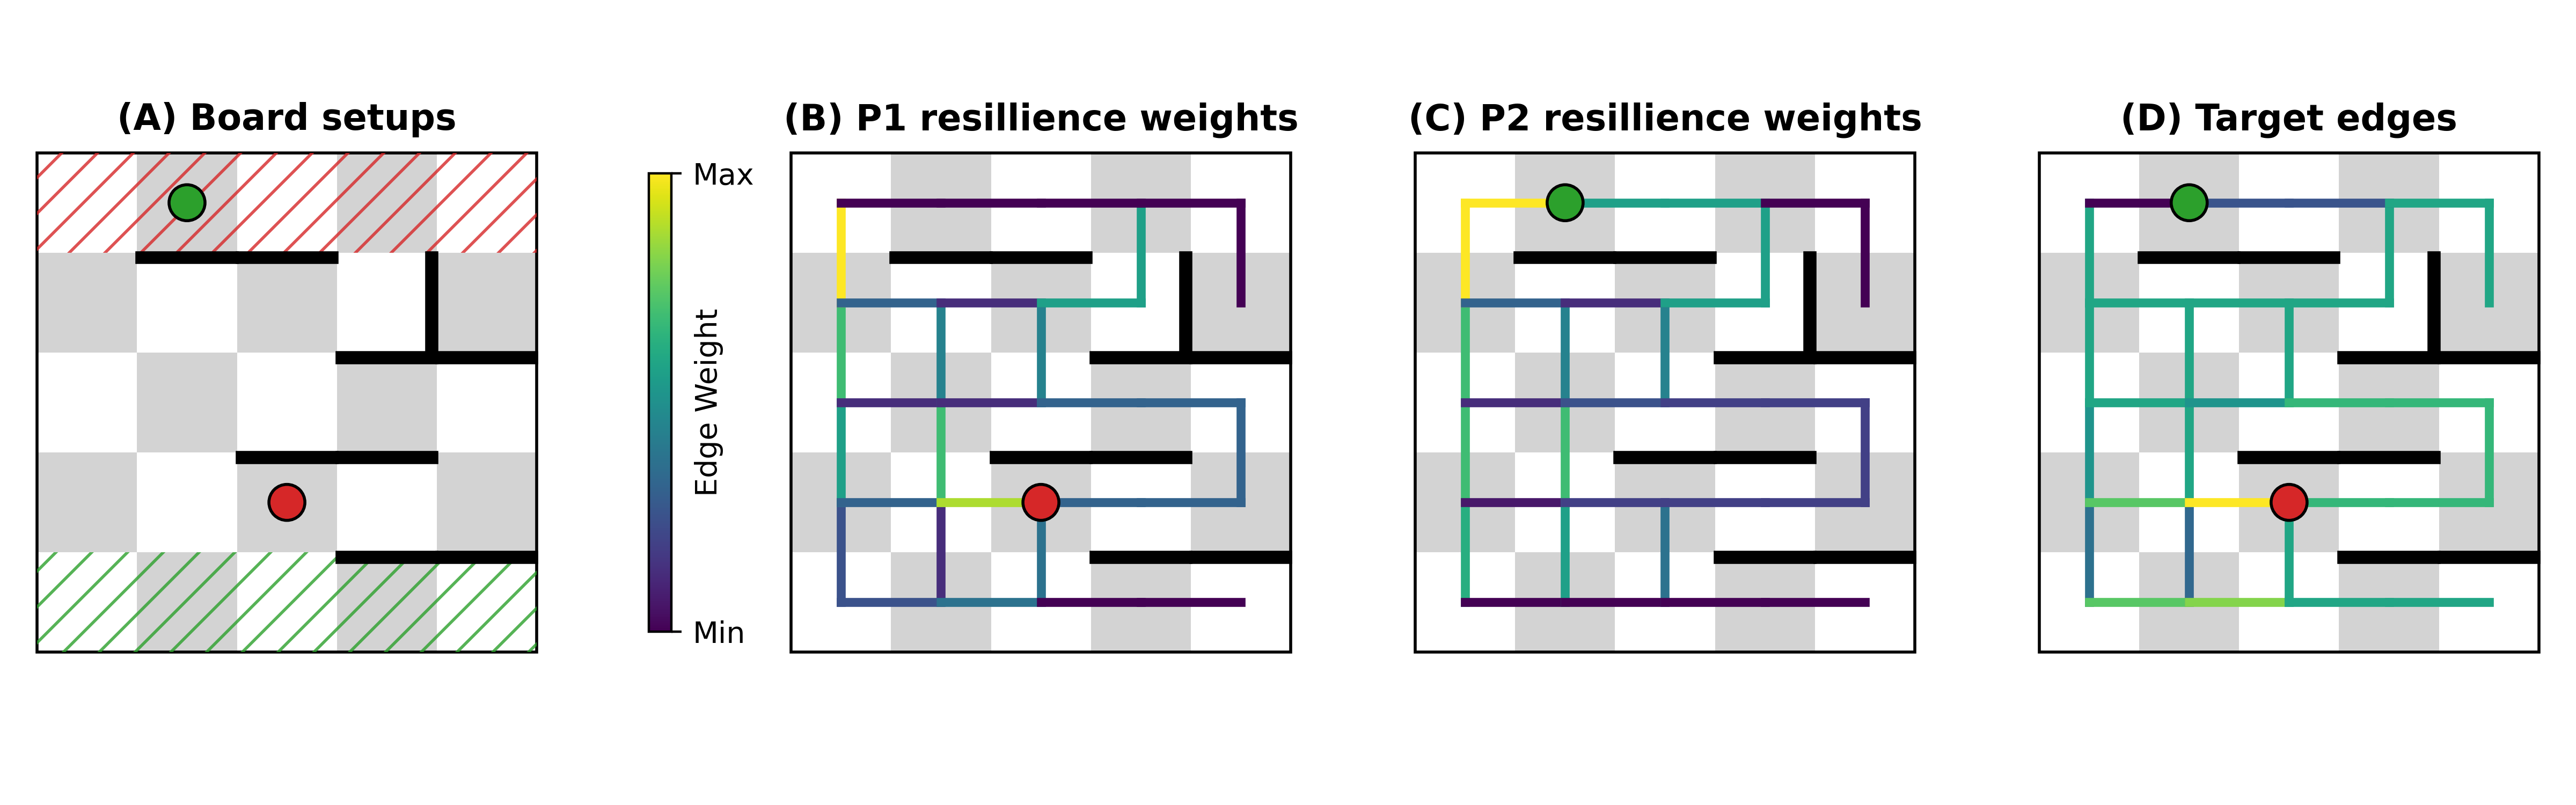
\includegraphics[width=\linewidth]{path_figure.png}
    \caption{\textbf{Path resiliency.} \textbf{(A)} The current position of the board. Player 1 is red; Player 2 is orange; Walls are black lines. Hashed regions denote the area a player must reach to win. \textbf{(B, C)} Resiliency weights of players 1 and 2, respectively. Higher values indicate that the edge is harder to avoid when finding alternate shortests paths to the goal. \textbf{(D)} Player 1 resiliency weights minus player 2 resiliency weights. A high values indicates that the edge is very damaging to player 1 when blocked, while not damaging to player 2.}
    \label{fig:sample}
\end{figure}

\section{Discussion}
Discuss the implications of your findings. Keep paragraphs short and precise.

% \section{References}
% Cite your sources using \texttt{natbib} style: \cite{example}.

\bibliographystyle{naturemag}
\bibliography{references}

\end{document}

